To address the issues, our group developed a full-stack quiz application that allows students to answer questions, gain points, and earn rewards. In this section, we will discuss the system architecture, the database design, and the implementation details of our application.
\subsection{System Architecture}
Our app is built with the client-server architecture, with the front end being implemented in React.js, and the backend being implemented in Express.js. The backend communicates with the database, which is implemented using a Microsoft SQL Server (MSSQL). Authentication and session management is handled using an Express session, with the user id being stored on the server rather than on the front end in order to prevent tampering. The front end and the backend communicate via RESTful API requests, which Express handles via the Express router, communicating with the backend and returning the proper results back to the client.
\begin{figure}[H]
    \centering
    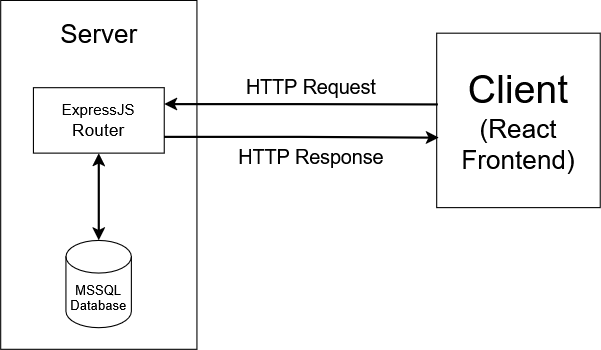
\includegraphics[width=0.7\linewidth]{PUT INDIVIDUAL SECTIONS HERE/images/clientServer(2).png}
    \caption{Client-Server Architecture of Quiz App}
    \label{client-server}
\end{figure}

\subsection{Data Modeling}
We designed our relational database schema to support users, classes, quizzes, questions, answers, and rewards. Users are able to join classes, earn points by taking quizzes associated with those classes, and then can use those points to redeem rewards.

\begin{figure}[H]
    \centering
    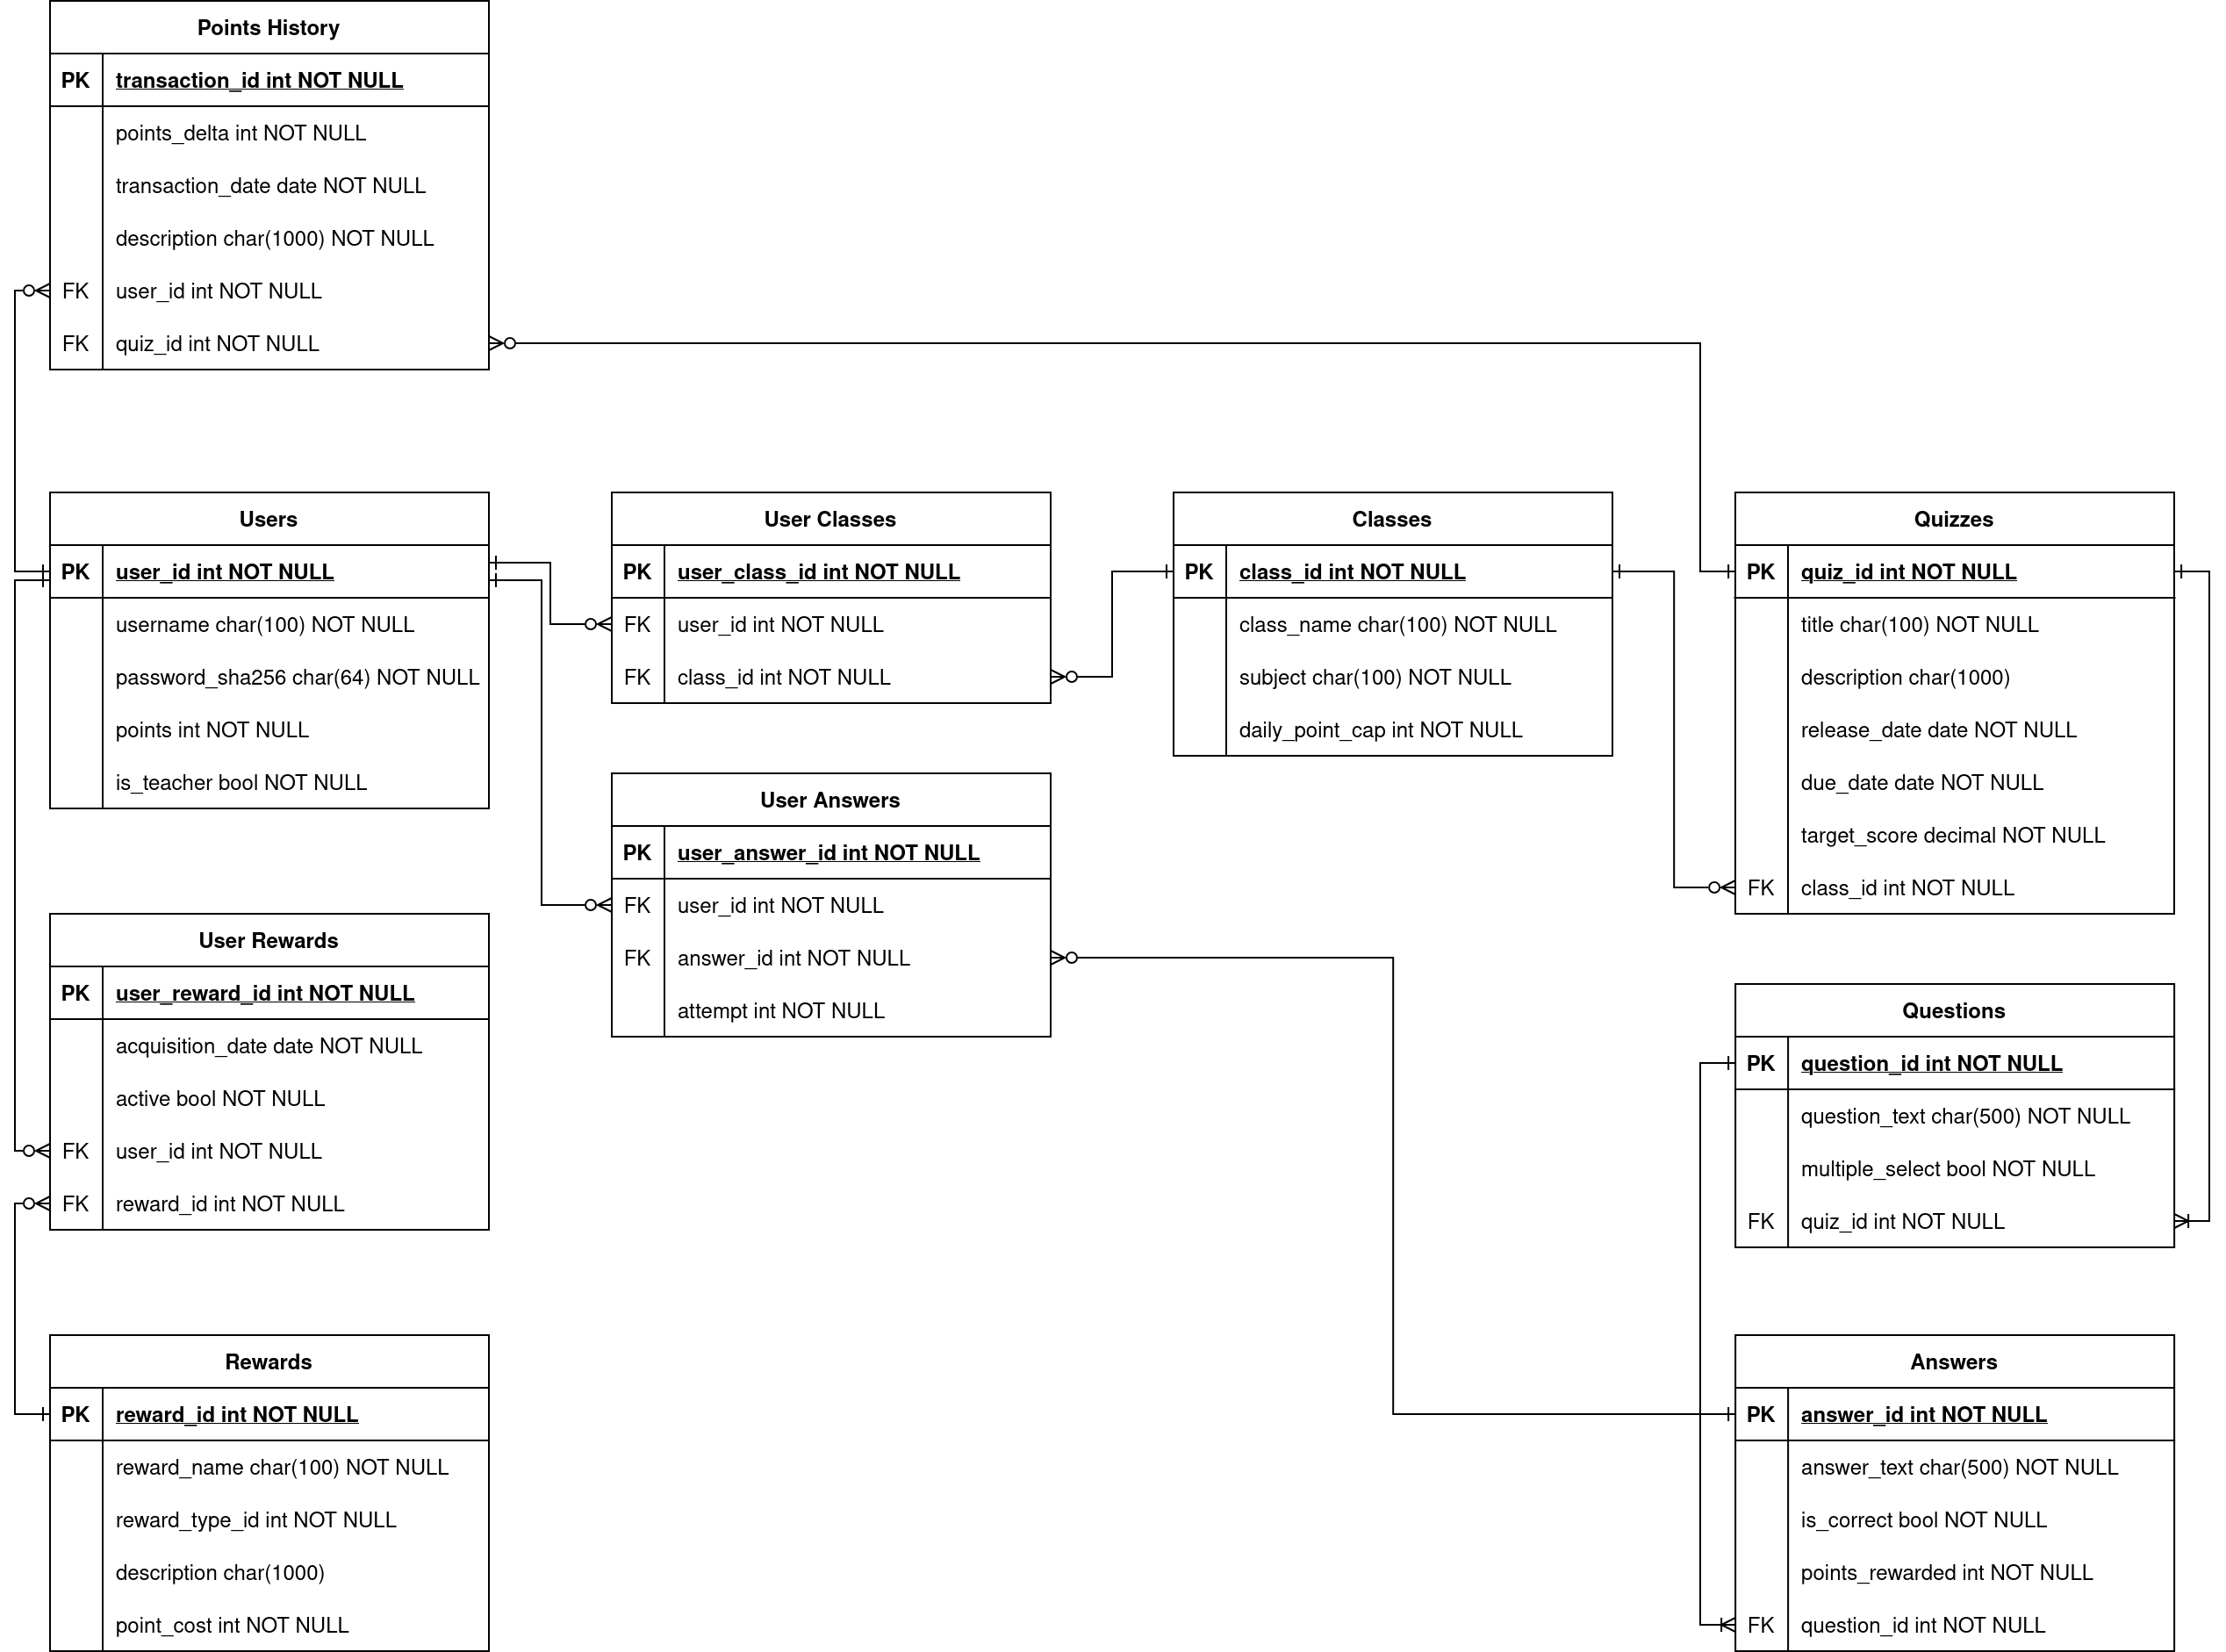
\includegraphics[width=0.7\linewidth]{PUT INDIVIDUAL SECTIONS HERE/images/466_ER_Diagram.drawio.png}
    \caption{Entity-Relationship Diagram for Database Schema}
    \label{ER-diagram}
\end{figure}

\subsection{Component Structure}
Our front end is built using React, which allows us to break up our app into modular components that each handle different functionality, making the app easier to maintain.
\begin{figure}[H]
    \centering
    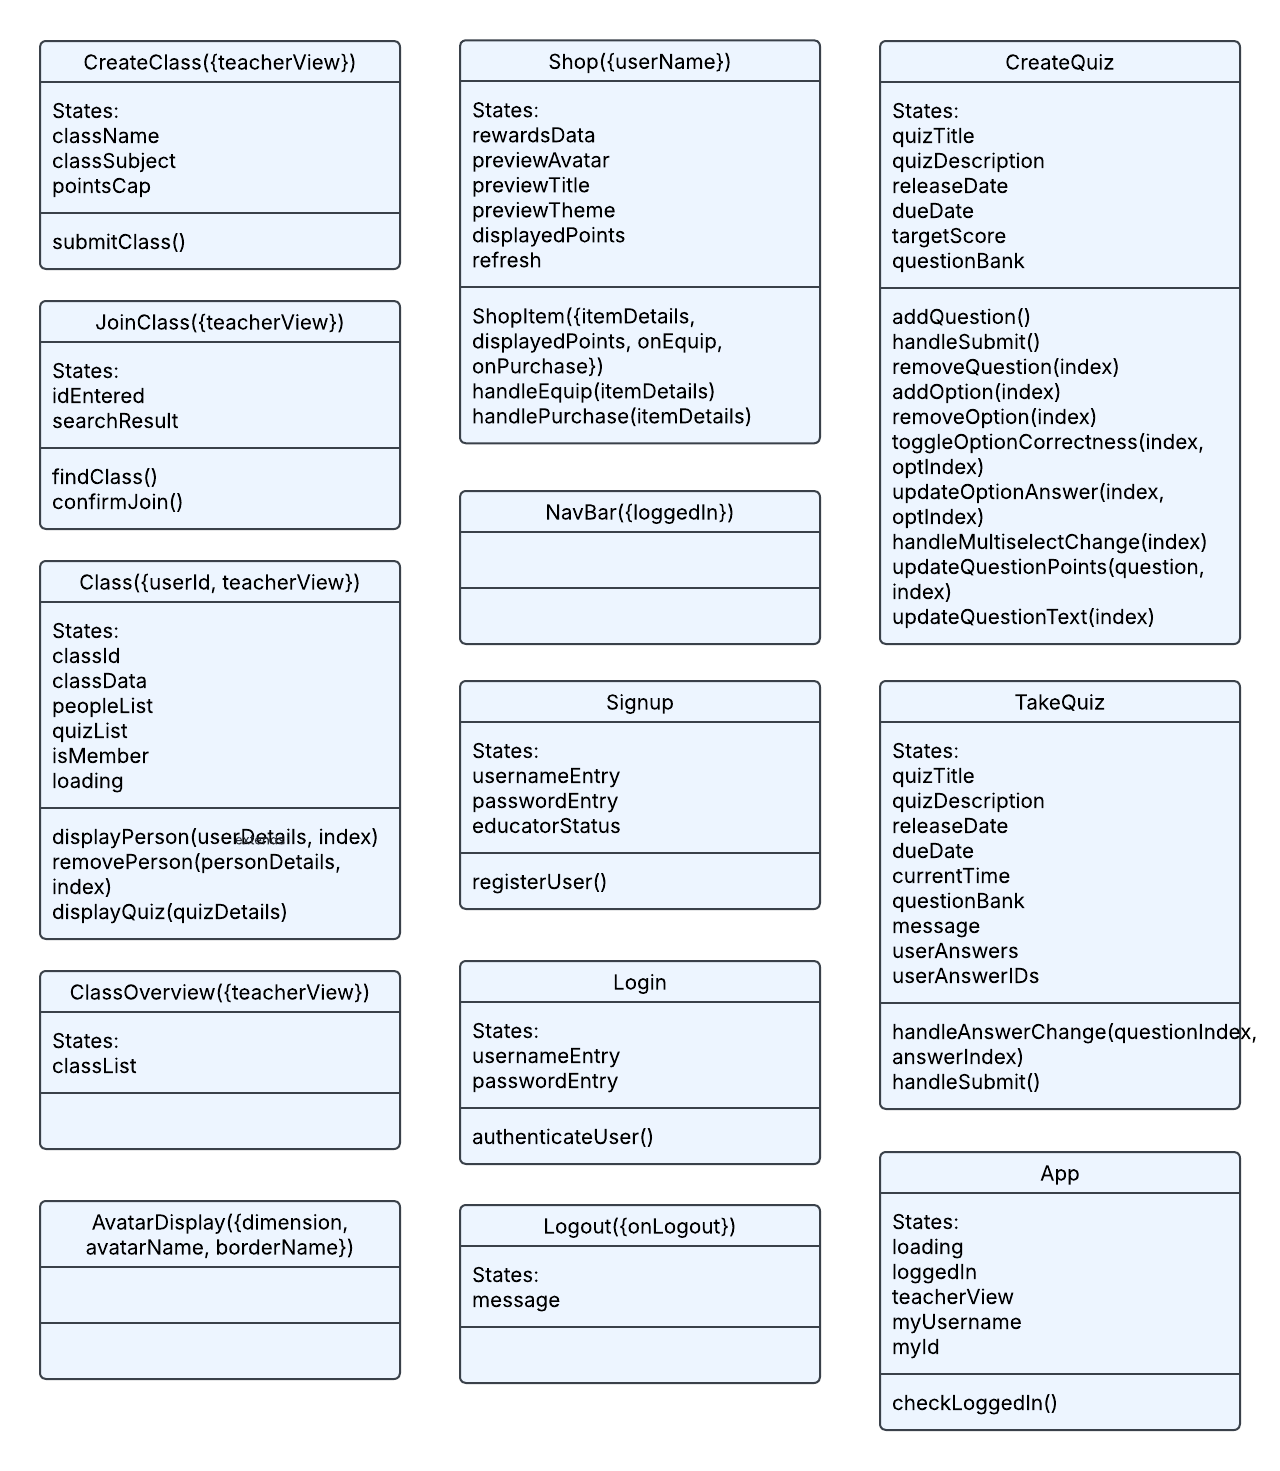
\includegraphics[width=0.7\linewidth]{PUT INDIVIDUAL SECTIONS HERE/images/UML_class.png}
    \caption{UML diagram that displays React components, states, and methods}
    \label{fig:enter-label}
\end{figure}
This diagram shows a high-level snapshot of some of the key components, including:
\begin{itemize}
    \item App - Manages global state, including login and authentication.
    \item CreateQuiz - Provides question/answer editing functionality.
    \item TakeQuiz - Renders quiz content, tracks answers, and submits completed attempts to backend.
    \item Shop - Handles reward purchasing and activation.
\end{itemize}
Business logic is handled inside each component, and most user actions result in fetch() calls to endpoints defined by the Express.js router.

\subsection{Application Walkthrough}
There are two main users that use the app, their workflows are shown below.
\subsubsection{Students}
\begin{enumerate}
    \item Students enter a class code in the JoinClass component.
    \begin{figure}[h]
        \centering
        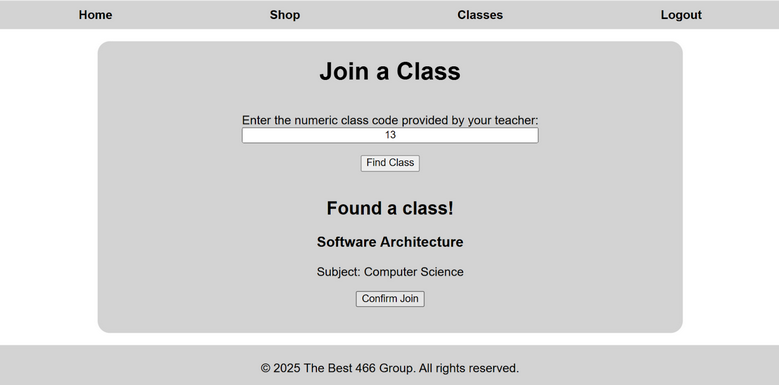
\includegraphics[width=0.7\linewidth]{PUT INDIVIDUAL SECTIONS HERE/images/joinClass.png}
        \caption{Join Class component}
        \label{join-class}
    \end{figure}
        \item Students can take quizzes assigned to them by their teachers, earning points with every correct answer.
    \begin{figure}[H]
        \centering
        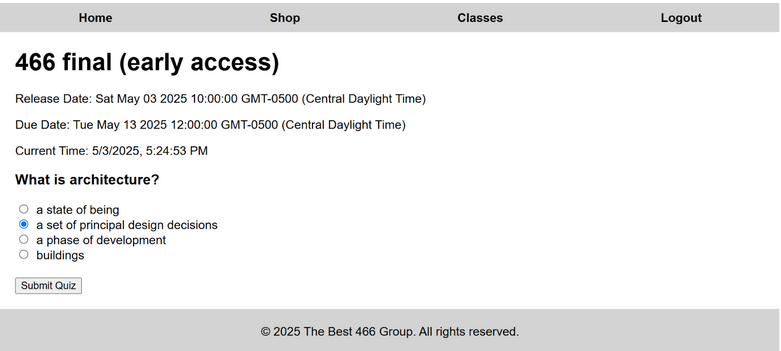
\includegraphics[width=0.7\linewidth]{PUT INDIVIDUAL SECTIONS HERE/images/TakeQuiz.png}
        \caption{Take Quiz component}
        \label{take-quiz}
    \end{figure}
        \item Students can then spend their accumulated points in the shop, earning customization features such as avatars.
\begin{figure}[H]
    \centering
    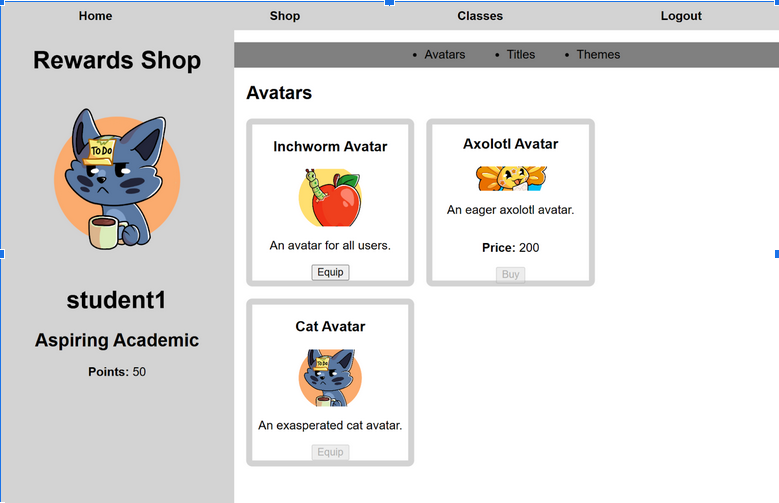
\includegraphics[width=0.7\linewidth]{PUT INDIVIDUAL SECTIONS HERE/images/Shop.png}
    \caption{Shop component}
    \label{Shop}
\end{figure}
\end{enumerate}
\subsubsection{Teachers}
\begin{enumerate}
    \item Teachers use the CreateClass component to define class name, subject, and daily point caps.
    \begin{figure}[h]
        \centering
        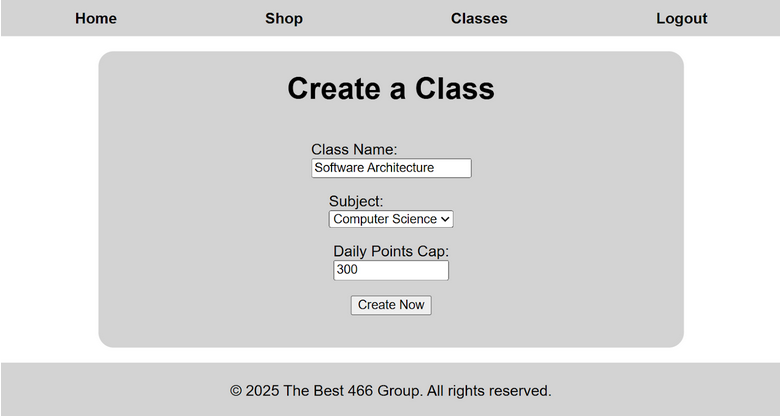
\includegraphics[width=0.7\linewidth]{PUT INDIVIDUAL SECTIONS HERE/images/createClass.png}
        \caption{Create Class component}
        \label{fig:enter-label}
    \end{figure}
        \item Teachers can view their students in with the ClassOverview component.
    \begin{figure}[H]
        \centering
        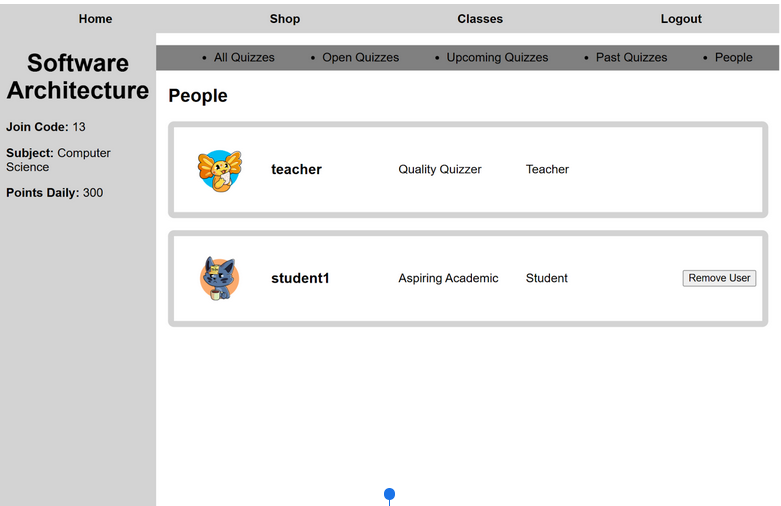
\includegraphics[width=0.7\linewidth]{PUT INDIVIDUAL SECTIONS HERE/images/classOverview.png}
        \caption{Class Overview component}
        \label{class-overview}
    \end{figure}
        \item Teachers can define quizzes with multiple questions with the CreateQuiz component. These questions support both single correct answer and multiple correct answers.
    \begin{figure}[H]
        \centering
        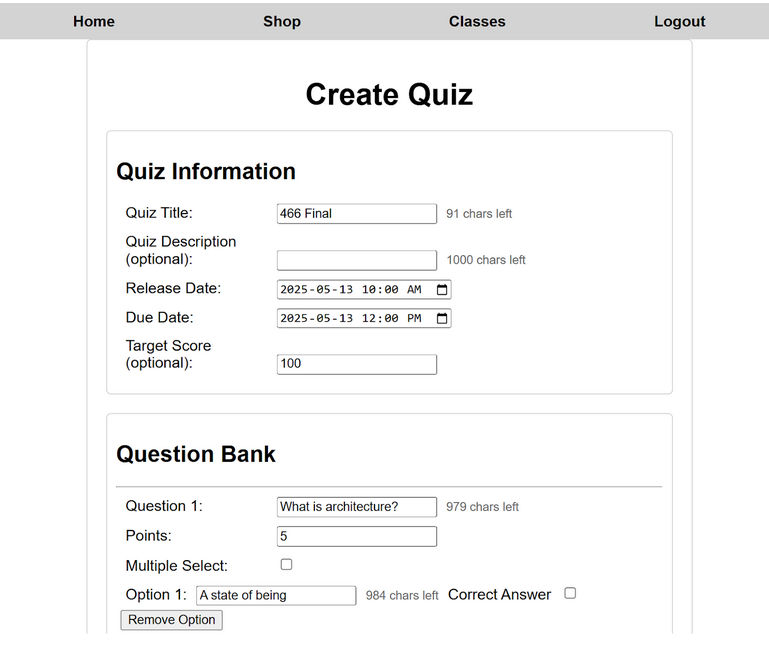
\includegraphics[width=0.7\linewidth]{PUT INDIVIDUAL SECTIONS HERE/images/createQuiz.png}
        \caption{Create Quiz component}
        \label{create-quiz}
    \end{figure}
        
\end{enumerate}
\subsection{Merit}
This tool successfully solves a number of problems mentioned in our background section. By allowing teachers the ability to create custom quizzes, teachers can successfully emphasize certain points in the curriculum, improving learning while simultaneously making life easier for teachers. For students, our app successfully supports the gamification of studying by allowing students to earn rewards for studying, turning it into a fun task rather than a chore. Our app also supports studying over time rather than cramming all at once with the introduction of a daily point cap. By introducing the cap, it encourages students to complete the quizzes on multiple days, rather than on a single day, in order to maximize their total points. Overall, our app reduces overhead for teachers, enhances student engagement, and supports classroom management.


